\documentclass[12pt]{article}
\usepackage[utf8]{inputenc}
\usepackage{geometry}
\geometry{letterpaper, margin=0.25in}
\usepackage{graphicx} 
\usepackage{parskip}
\usepackage{booktabs}
\usepackage{array} 
\usepackage{paralist} 
\usepackage{verbatim}
\usepackage{subfig}
\usepackage{fancyhdr}
\usepackage{sectsty}
\usepackage[shortlabels]{enumitem}

\pagestyle{fancy}
\renewcommand{\headrulewidth}{0pt} 
\lhead{}\chead{}\rhead{}
\lfoot{}\cfoot{\thepage}\rfoot{}

%%% ToC (table of contents) APPEARANCE
\usepackage[nottoc,notlof,notlot]{tocbibind} 
\usepackage[titles,subfigure]{tocloft}
\renewcommand{\cftsecfont}{\rmfamily\mdseries\upshape}
\renewcommand{\cftsecpagefont}{\rmfamily\mdseries\upshape} %

\usepackage{amsmath}
\usepackage{amssymb}
\usepackage{mathtools}
\usepackage{empheq}
\usepackage{xcolor}
\usepackage{bbm}
\usepackage{tikz}
\usepackage{pgfplots}
\usepackage{tikz-cd}
\pgfplotsset{compat=1.18}

\newcommand{\ans}[1]{\boxed{\text{#1}}}
\newcommand{\vecs}[1]{\langle #1\rangle}
\renewcommand{\hat}[1]{\widehat{#1}}

\renewcommand{\P}{\mathbb{P}}
\newcommand{\R}{\mathbb{R}}
\newcommand{\E}{\mathbb{E}}
\newcommand{\Z}{\mathbb{Z}}
\newcommand{\N}{\mathbb{N}}
\newcommand{\Q}{\mathbb{Q}}
\newcommand{\C}{\mathbb{C}}

\newcommand{\ind}{\mathbbm{1}}
\newcommand{\qed}{\quad \blacksquare}

\newcommand{\brak}[1]{\left\langle #1 \right\rangle}
\newcommand{\bra}[1]{\left\langle #1 \right\vert}
\newcommand{\ket}[1]{\left\vert #1 \right\rangle}

\newcommand{\abs}[1]{\left\vert #1 \right\vert}
\newcommand{\mfX}{\mathfrak{X}}
\newcommand{\ep}{\varepsilon}

\newcommand{\Ec}{\mathcal{E}}
\newcommand{\A}{\mathcal{A}}
\newcommand{\F}{\mathcal{F}}
\newcommand{\Cc}{\mathcal{C}}
\newcommand{\B}{\mathcal{B}}
\newcommand{\M}{\mathcal{M}}
\newcommand{\X}{\chi}
\renewcommand{\L}{\mathcal{L}}

\newcommand{\sub}{\subseteq}
\newcommand{\st}{\text{ s.t. }}
\newcommand{\card}{\text{card }}
\renewcommand{\div}{\vspace*{10pt}\hrule\vspace*{10pt}}
\newcommand{\surj}{\twoheadrightarrow}
\newcommand{\inj}{\hookrightarrow}
\newcommand{\biject}{\hookrightarrow \hspace{-8pt} \rightarrow}
\renewcommand{\bar}[1]{\overline{#1}}
\newcommand{\overcirc}[1]{\overset{\circ}{#1}}
\newcommand{\diam}{\text{diam }}

\renewcommand{\Re}{\text{Re}\,}
\renewcommand{\Im}{\text{Im}\,}
\newcommand{\sign}{\text{sign}\,}

\newcommand*{\tbf}[1]{\ifmmode\mathbf{#1}\else\textbf{#1}\fi}

\usepackage{tcolorbox}
\tcbuselibrary{breakable, skins}
\tcbset{enhanced}
\newenvironment*{tbox}[2][gray]{
    \begin{tcolorbox}[
        parbox=false,
        colback=#1!5!white,
        colframe=#1!75!black,
        breakable,
        title={#2}
    ]}
    {\end{tcolorbox}}

\newenvironment*{exercise}[1][red]{
    \begin{tcolorbox}[
        parbox=false,
        colback=#1!5!white,
        colframe=#1!75!black,
        breakable
    ]}
    {\end{tcolorbox}}

\newenvironment*{proof}[1][blue]{
\begin{tcolorbox}[
    parbox=false,
    colback=#1!5!white,
    colframe=#1!75!black,
    breakable
]}
{\end{tcolorbox}}

\title{APMA 1360 Homework 1}
\author{Milan Capoor}
\date{31 Jan 2025}

\begin{document}
\maketitle

\section*{Problem 1 - ODEs on the Real Line}
For each of (i)-(vi) below, find a continuously differentiable function $f : \R \to \R$ such that the differential equation $\dot u = f (u)$ has the stated properties or, if there is no such function, explain in detail (with a proof or a precise
argument) why not. If possible, give an explicit expression of the function; otherwise, sketch its graph.

\begin{enumerate}[label=(\roman*)]
    \item Every real number is an equilibrium.
          \color{blue}
          $\boxed{f = 0}$
          \color{black}

    \item Every integer is an equilibrium, and there are no other fixed points besides those.
          \color{blue}
          $\boxed{f(u) = \sin(\pi u)}$
          \color{black}

    \item There are exactly two equilibria, and both of them are stable.

          \color{blue}
          Impossible. If there are exactly two equilibria, then $f$ has two roots (say $u_1, u_2$ and WLOG assume $u_1 < u_2$).

          As it is an equilibrium, $f(u_1) = 0$. By assumption, $u_1$ is stable so $f'(u_1) < 0$.

          CASE 1: $f'(u) < 0$ for all $u$.

          But then, $f$ is strictly decreasing so $\forall \ep > 0$, $f(u_1 + \ep) < f(u_1) = 0 $.

          In particular, let $\ep = u_2 - u_1 > 0$. then $f(u_1 + \ep) = f(u_2) < f(u_1) = 0 \implies f(u_2) < 0$ which contradicts the fact that $u_2$ is an equilibrium.

          CASE 2: $\exists I \sub \R$ such that $f'(t) \geq 0$ for $t \in I$.

          If $u_2 \in I$, then $u_2$ is not a stable equilibrium. Contradiction.

          If $u_2 \notin I$ and $f$ is not strictly decreasing everywhere (Case 1), then since $f \in C^1$, $u_1 < u_2$, $f(u_1 + \ep) < 0$, and $f(u_2) = 0$, by the Intermediate Value Theorem, $\exists u_3 \in (u_1, u_2)$ such that $f(u_3) = 0$. Contradiction.

          \color{black}


    \item There are no equilibria.
          \color{blue}
          $\boxed{f = 1}$
          \color{black}

    \item The phase diagram looks as shown in the picture below:

          \begin{center}
              \begin{tikzpicture}
                  \node (0, 0) {\includegraphics[width=0.8\textwidth]{Images/1-phase-diagram.png}};
                  \node[blue] at (-4.2, -0.5) {$u_1$};
                  \node[blue] at (-1.3, -0.5) {$u_2$};
                  \node[blue] at (2.5, -0.5) {$u_3$};
                  \node[blue] at (5.5, -0.5) {$u_4$};
              \end{tikzpicture}
          \end{center}

          \color{blue}
          We label the equilibria as $u_1 < u_2 < u_3 < u_4$. Then,
          \begin{itemize}
              \item $u_1$, $u_4$ are stable
              \item $u_2$ is a saddle point
              \item $u_3$ is unstable
          \end{itemize}

          Hence,
          \[f'(u_1) <0, \quad f'(u_2) = 0, \quad f'(u_3) > 0, \quad f'(u_4) < 0\]

          So, the graph of $f$ must resemble
          \begin{center}
              \color{black}
              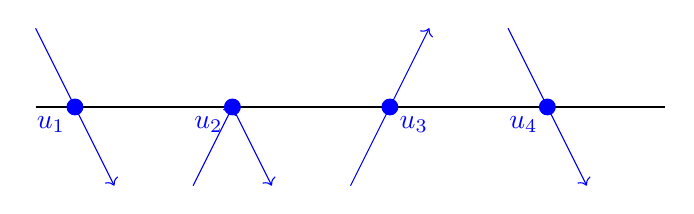
\begin{tikzpicture}
                  \draw (0,0) -- (8,0); %axis

                  \draw[->, blue] (0, 1) -- (1, -1) node[midway] (u1) {};
                  \draw[fill, blue] (u1) circle (0.1) node[below left] {$u_1$};

                  \draw[fill, blue] (2.5, 0) circle (0.1) node[below left] {$u_2$};
                  \draw[->, blue] (2, -1) -- (2.5, 0);
                  \draw[->, blue] (2.5, 0) -- (3, -1);



                  \draw[->, blue] (4, -1) -- (5, 1) node[midway] (u3) {};
                  \draw[fill, blue] (u3) circle (0.1) node[below right] {$u_3$};

                  \draw[->, blue] (6, 1) -- (7, -1) node[midway] (u4) {};
                  \draw[fill, blue] (u4) circle (0.1) node[below left] {$u_4$};
              \end{tikzpicture}
          \end{center}

          One possible function is $\boxed{f(u) = -u(u-1)^2 (u-3)(u-4)}$:

          \begin{center}
              \color{black}
              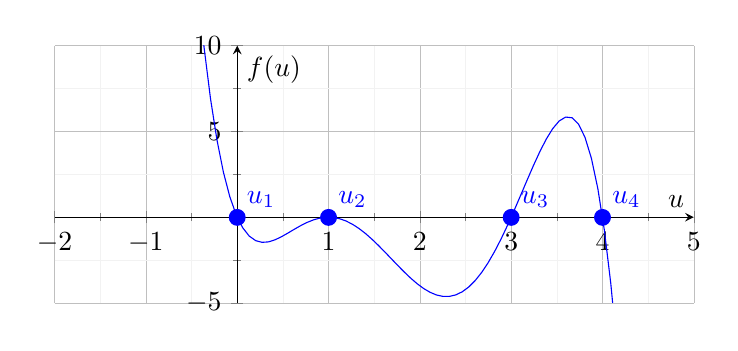
\begin{tikzpicture}
                  \begin{axis}
                      [
                          axis lines=middle,
                          ymin=-5, ymax=10,
                          xmin=-2, xmax=5,
                          xlabel=$u$,
                          ylabel=$f(u)$,
                          grid=both,
                          minor tick num=1,
                          grid style={line width=.1pt, draw=gray!10},
                          major grid style={line width=.2pt,draw=gray!50},
                          width=0.8\textwidth,
                          height=0.4\textwidth,
                          samples=100
                      ]
                      \addplot[domain=-1:6, blue] {-x*(x-1)^2*(x-3)*(x-4)};
                      \coordinate (u1) at (axis cs:0,0);
                      \coordinate (u2) at (axis cs:1,0);
                      \coordinate (u3) at (axis cs:3,0);
                      \coordinate (u4) at (axis cs:4,0);

                  \end{axis}
                  \draw[fill, blue] (u1) circle (0.1) node[above right] {$u_1$};
                  \draw[fill, blue] (u2) circle (0.1) node[above right] {$u_2$};
                  \draw[fill, blue] (u3) circle (0.1) node[above right] {$u_3$};
                  \draw[fill, blue] (u4) circle (0.1) node[above right] {$u_4$};
              \end{tikzpicture}
          \end{center}

          \color{black}

    \item The differential equation has a solution $u(t)$ that is periodic in $t$: there is a $T > 0$ with $u(t + T ) = u(t)$ for all $t$, but $u(t)$ is not an equilibrium (that is, not a constant function).

          \color{blue}

          Impossible. Suppose there exists such a periodic solution $u$ for such an $f$. Consider a point $u(t_0)$. By periodicity, $u(t_0) = u(t_0 + T)$.

          Since $f \in C^1$, $u \in C^2$ and by Rolle's Theorem, $\exists t^* \in (t_0, t_0 + T)$ such that
          \[f(u(t^*)) = u'(t^*) = \frac{u(t_0 + T) - u(t_0)}{T} = 0\]

          If $f(u(t)) = 0$ for all $t \in (t_0, t_0 + T)$, hence $u(t)$ is an equilibrium. Contradiction of assumption.

          Otherwise, $u(t^*)$ is an equilibrium. If $f$ is decreasing at $u(t^*)$, then the equilibrium is stable, hence $u(t)$ is constant in $t$ - Contradiction.

          If $f$ is increasing at $u(t^*)$, then since $u$ is periodic, there must exist some other equilibrium point where $f$ is decreasing, again leading to a stable equilibrium.
          \color{black}
\end{enumerate}



\pagebreak
\section*{Problem 2 - Logistic model}

The differential equation
\[\frac{du}{dt} = ru\left(1 - \frac{u}{K}\right) - \mu u\]
serves as a model for a population of fish with harvesting: $u(t)$ is the size of the population at time $t, r > 0$ is the
growth rate of fish at small population levels, $K > 0$ is called the carrying capacity, and $\mu \geq 0$ is the percentage of
fish caught per unit time interval.
\begin{enumerate}
    \item Analyze this model mathematically: find all equilibria, determine their stability, and identify all bifurcation
          points (if any) at which the number of equilibria changes as a function of the fishing rate $\mu$.

          \color{blue}
          Let $f(u) = ru\left(1 - \frac{u}{K}\right) - \mu u$. Then, the equilibria are given by
          \[u_1 = 0, \quad u_2 = K(1 -\frac{\mu}{r})\]
          (these are the only equilibria as $f$ is quadratic in $u$.)

          Further,
          \[f'(u) = r - \mu - \frac{2r}{K}u\]
          and
          \[f'(u_1) = r - \mu, \quad f'(u_2) = r - \mu - 2(r - \mu) = \mu - r\]

          Hence,
          \begin{itemize}
              \item $u_1 = 0$ is stable for $\mu > r$, unstable for $\mu < r$, and undetermined for $\mu = r$.\
              \item $u_2 = \frac{K}{r}(r -\mu)$ is stable for $r > \mu$. For $\mu > r$, $u_2 = K(1 - \frac{\mu}{r}) < 0$ which is impossible. For $\mu = r$, $u_2 = 0$ and there exists only one equilibrium.
          \end{itemize}

          By the above argument, $\mu = r$ is a bifurcation point since for $\mu < r$, there are two equilibria and for $\mu > r$, there is only one equilibrium.

          \color{black}


    \item Draw the bifurcation diagram with respect to $(\mu, u).$

          \begin{center}
              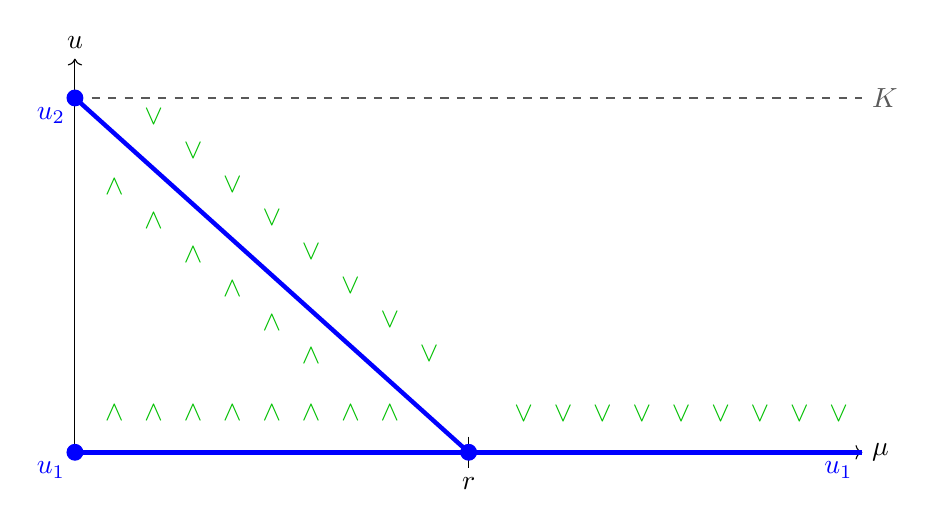
\begin{tikzpicture}
                  \draw[->] (0, 0) -- (10, 0) node[right] {$\mu$};
                  \draw[->] (0, 0) -- (0, 5) node[above] {$u$};

                  \draw (5, 0.2) -- (5, -0.2) node[below] {$r$};
                  \draw[dashed, gray!70!black] (0, 4.5) -- (10, 4.5) node[right] {$K$};

                  \draw[blue, fill] (0, 0) circle (0.1) node[below left] {$u_1$};
                  \draw[blue, ultra thick] (0, 0) -- (10, 0);

                  \draw[blue, fill] (0, 4.5) circle (0.1) node[below left] {$u_2$};
                  \draw[blue, ultra thick] (0, 4.5) -- (5, 0) ;

                  \draw[blue, fill] (5, 0) circle (0.1);
                  \node[below left, blue] at (10, 0) {$u_1$};

                  \foreach \x in {1, ..., 8} {
                          \node[green!75!black] at (0.5*\x, 0.5) {$\wedge$};
                      }

                  \foreach \x in {1, ..., 9} {
                          \node[green!75!black] at (5.2+0.5*\x, 0.5) {\rotatebox{180}{$\wedge$}};
                      }

                  \foreach \x in {1, ..., 6} {
                          \node[green!75!black] at (0.5*\x, 3.8-0.43*\x) {$\wedge$};
                      }

                  \foreach \x in {1, ..., 8} {
                          \node[green!75!black] at (0.5+0.5*\x, 4.7-0.43*\x) {\rotatebox{180}{$\wedge$}};
                      }
              \end{tikzpicture}
          \end{center}
    \item Discuss the meaning of the carrying capacity $K$ and identify which equilibria are meaningful with respect to
          the underlying application, where $u(t)$ captures the size of the fish population. Discuss the implications of your analysis for the underlying application of fishing/harvesting of fish.

          \color{blue}
          If there were no fishing ($\mu = 0$), then since $u_1$ is unstable and $u_2$ is stable, the fish population would stabilize at $u = K$. As we introduce fishing ($\mu \nearrow$), the equilibrium solution $K - \frac{K}{r}\mu$, representing a stable fish population, decreases. Hence, if the fishing rate $\mu$ exceeds the growth rate $r$, then the fish population will die out. If, instead, $0 < \mu < r$, then the fish population will stabilize at a lower level than $K$ and the fishing rate will be sustainable.
          \color{black}
\end{enumerate}

\pagebreak

\section*{Problem 3 - Stability of Equilibria}

In your own words, write down a concise definition of when we call an equilibrium stable.

\color{blue}
For a differential equation of the form $\dot u = f(u)$, $u^*$ is an equilibrium point if $f(u^*) = 0$. We say that $u^*$ is a stable equilibrium if $\exists \ep > 0$ such that $\forall u_i \in B_\ep(u^*)$, $\lim_{t\to\infty} u(t) = u^*$ for all solutions $u(t)$ with $u(0) = u_i$.


\end{document}